\subsection{The fundamental domain and the tessellation of the halfplane}

We have seen in Remark~\ref{rem_NatureMoebius} that considering M�bius transformations as meromorphic functions $\EC \to \EC$ very naturally induces a group action of $\PGL{\C}$ on $\EC$. Clearly this group action is also given for any subgroup of $\PGL{\C}$ and in particular for the modular group. 

For the following it will be convenient to write modular transformations in matrix form and the elements $z \in \EC$ as quotients $z = u/v$ for suitable $u,v \in \C$, not both zero. A formal quotient $u/0$ will be identified with $\infty$. In this notation, for a modular transformation $A = \smallmat{a}{b}{c}{d} \in \PSL{\Z}$ and $u/v \in \EC$ the mentioned group action is given by
\begin{equation}
\label{eqn_ModGrpAction}
A \ \frac{u}{v} := \frac{a u + b v}{c u + d v}
\end{equation}
We call two points $z, w \in \EC$ \emph{equivalent}, if and only if there is a modular transformation $A \in \PSL{\Z}$ with $A z = w$ and we write  $z \sim w$. The equivalence class (\emph{orbit}) of a point $u/v \in \EC$ is given by 
\begin{equation*}
\left[\frac{u}{v}\right]_\sim = 
\setdefsz{\bigg}{\frac{a u + b v}{c u + d v} \in \EC}{\mat{a}{b}{c}{d} \in \PSL{\Z}} \in \EC / \sim.
\end{equation*}
We now wish to find a system of representatives for $\EC/\sim$, in other words, we want to define exactly one representative $u_0/v_0$ for each orbit $[u/v]_\sim$. One approach for this could be to fix $u,v \in \C$, not both zero, then to choose from the set
\begin{equation}
\label{eqn_FunDomLuv}
O_{u,v} := \setdefsz{\bigg}{\cvec{a u + b v}{c u + d v} \in \C^2}{\mat{a}{b}{c}{d} \in \SL{\Z}}
\end{equation}
one vector $(u_0, v_0)$ with minimal $\eucnorm{\cdot}$-norm and to declare $u_0/v_0$ as the representative for $[u/v]_\sim$. The problem with this is that such a choice may not always be possible, because $L_{u,v}$ may in general contain vectors of arbitrary small $\eucnorm{\cdot}$-norm. However, if $u \conj{v} \notin \R$,  then the set 
\begin{equation*}
L_{u,v} := \setdef{a u + b v \in \C}{a,b \in \Z}
\end{equation*}
forms a lattice in $\C$.\footnote{The condition $u \conj{v} \notin \R$ is equivalent to $v \ne 0$ and $\Im{u/v} \ne 0$.} For this reason there exists a positive lower bound $m$ satisfying $0 < m \le \abs{z}$ for all $z \in L_{u,v} \setminus \{0\}$. Obviously $O_{u,v} \subseteq (L_{u,v})^2$ and $(0,0) \notin O_{u,v}$, which is why $m$ is also a lower bound for the $\eucnorm{\cdot}$-norm of the elements of $O_{u,v}$:
\begin{equation*}
0 < m \le \eucnorm{x} \quad \forall x \in O_{u,v}.
\end{equation*}

\begin{figure}
\centering
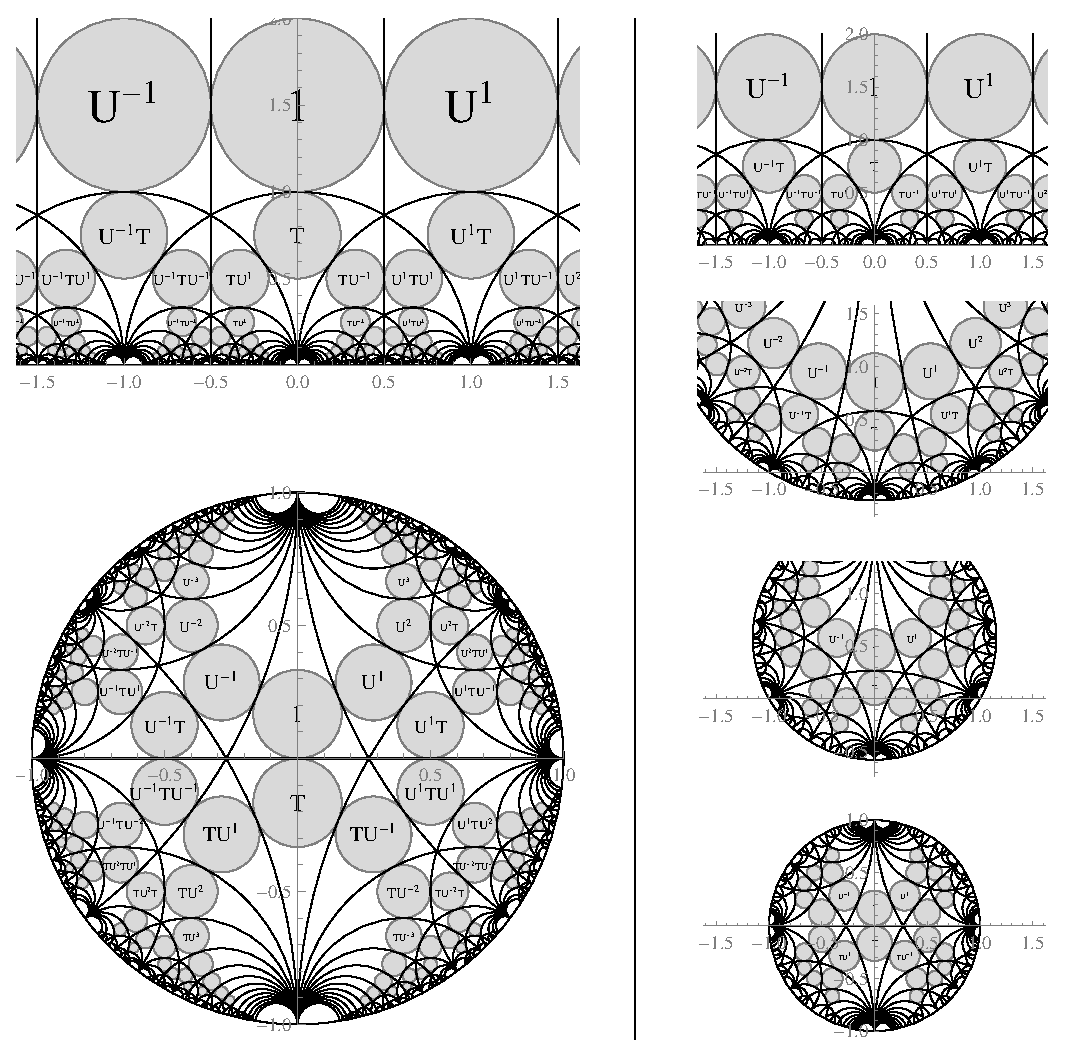
\includegraphics[width=\textwidth]{figures/modular-tiling-1}
\caption{The tessellation of the upper halfplane.}
\label{fig_ModularTiling}
\end{figure}

\begin{figure}
\centering
\includegraphics[width=0.8\textwidth]{figures/modular-tiling-exp-fan}
\caption{The tessellation under the transformation $z \mapsto \exp(2 \pi \ii z)$.}
\label{fig_ModularTilingExpFan}
\end{figure}

\begin{figure}
\centering
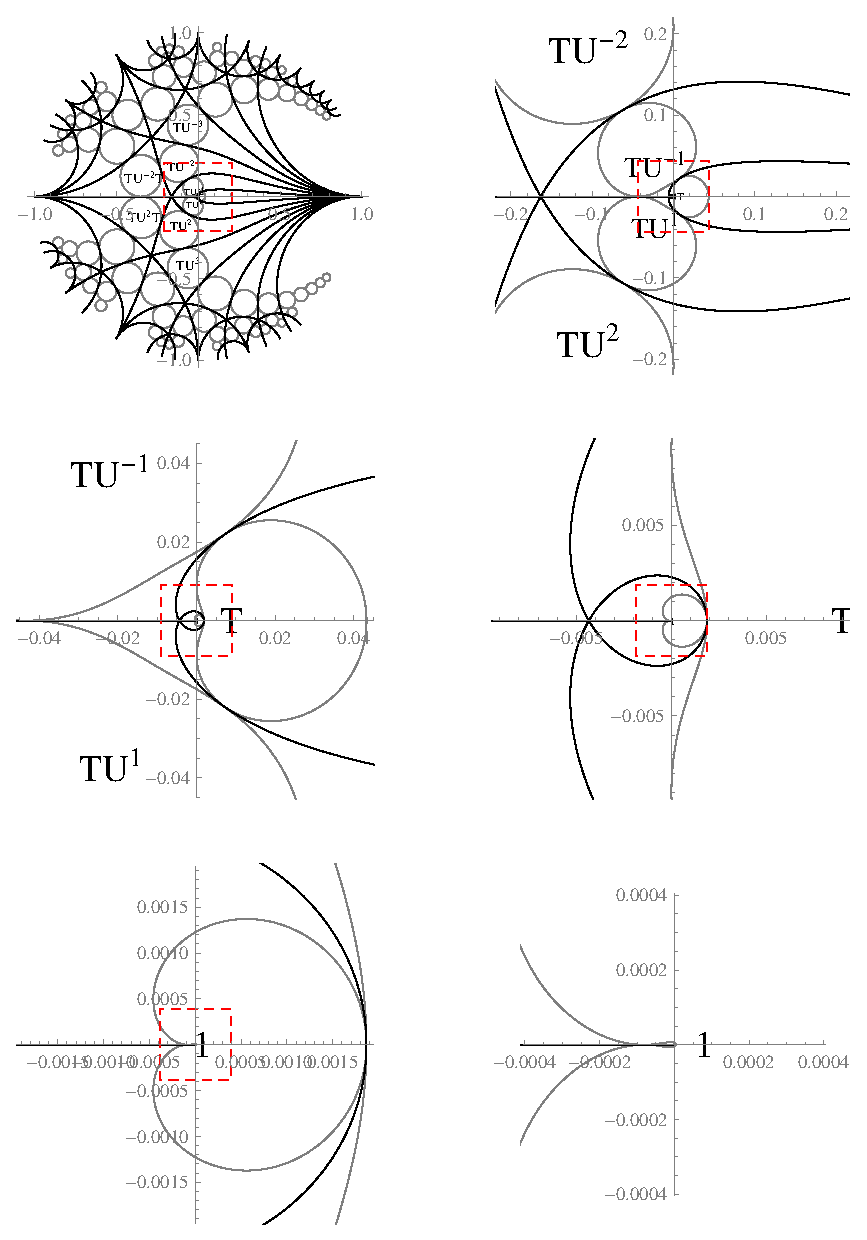
\includegraphics[width=0.8\textwidth]{figures/modular-tiling-exp-zoom}
\caption{The image of the modular tiling under the map $z \mapsto \exp(2 \pi \ii z)$ in the neighborhood of $\infty$.}
\label{fig_ModularTilingExpZoom}
\end{figure}

\todo{25}{Definition, description and figures}
